%% LyX 2.1.3 created this file.  For more info, see http://www.lyx.org/.
%% Do not edit unless you really know what you are doing.
\documentclass{article}\usepackage[]{graphicx}\usepackage[]{color}
%% maxwidth is the original width if it is less than linewidth
%% otherwise use linewidth (to make sure the graphics do not exceed the margin)
\makeatletter
\def\maxwidth{ %
  \ifdim\Gin@nat@width>\linewidth
    \linewidth
  \else
    \Gin@nat@width
  \fi
}
\makeatother

\definecolor{fgcolor}{rgb}{0.345, 0.345, 0.345}
\newcommand{\hlnum}[1]{\textcolor[rgb]{0.686,0.059,0.569}{#1}}%
\newcommand{\hlstr}[1]{\textcolor[rgb]{0.192,0.494,0.8}{#1}}%
\newcommand{\hlcom}[1]{\textcolor[rgb]{0.678,0.584,0.686}{\textit{#1}}}%
\newcommand{\hlopt}[1]{\textcolor[rgb]{0,0,0}{#1}}%
\newcommand{\hlstd}[1]{\textcolor[rgb]{0.345,0.345,0.345}{#1}}%
\newcommand{\hlkwa}[1]{\textcolor[rgb]{0.161,0.373,0.58}{\textbf{#1}}}%
\newcommand{\hlkwb}[1]{\textcolor[rgb]{0.69,0.353,0.396}{#1}}%
\newcommand{\hlkwc}[1]{\textcolor[rgb]{0.333,0.667,0.333}{#1}}%
\newcommand{\hlkwd}[1]{\textcolor[rgb]{0.737,0.353,0.396}{\textbf{#1}}}%

\usepackage{framed}
\makeatletter
\newenvironment{kframe}{%
 \def\at@end@of@kframe{}%
 \ifinner\ifhmode%
  \def\at@end@of@kframe{\end{minipage}}%
  \begin{minipage}{\columnwidth}%
 \fi\fi%
 \def\FrameCommand##1{\hskip\@totalleftmargin \hskip-\fboxsep
 \colorbox{shadecolor}{##1}\hskip-\fboxsep
     % There is no \\@totalrightmargin, so:
     \hskip-\linewidth \hskip-\@totalleftmargin \hskip\columnwidth}%
 \MakeFramed {\advance\hsize-\width
   \@totalleftmargin\z@ \linewidth\hsize
   \@setminipage}}%
 {\par\unskip\endMakeFramed%
 \at@end@of@kframe}
\makeatother

\definecolor{shadecolor}{rgb}{.97, .97, .97}
\definecolor{messagecolor}{rgb}{0, 0, 0}
\definecolor{warningcolor}{rgb}{1, 0, 1}
\definecolor{errorcolor}{rgb}{1, 0, 0}
\newenvironment{knitrout}{}{} % an empty environment to be redefined in TeX

\usepackage{alltt} 
\usepackage{ucs}
\usepackage[utf8x]{inputenc}
\usepackage[sc]{mathpazo}
\usepackage[T1]{fontenc}
\usepackage{geometry}

\newenvironment{uzdevums}[1][\unskip]{%
\vspace{3mm}
\noindent
\textbf{#1 uzdevums:}
\noindent}
{}

\geometry{verbose,tmargin=2.5cm,bmargin=2.5cm,lmargin=2.5cm,rmargin=2.5cm}
\setcounter{secnumdepth}{2}
\setcounter{tocdepth}{2}
\usepackage{url}
\usepackage[unicode=true,pdfusetitle,
 bookmarks=true,bookmarksnumbered=true,bookmarksopen=true,bookmarksopenlevel=2,
 breaklinks=false,pdfborder={0 0 1},backref=false,colorlinks=false]
 {hyperref}
\renewcommand{\abstractname}{Anotācija}
\hypersetup{
 pdfstartview={XYZ null null 1}}
\IfFileExists{upquote.sty}{\usepackage{upquote}}{}
\begin{document}




\title{Olimpiāžu pārskatos izmantotie apzīmējumi}

\author{}
\date{}

\maketitle

\begin{abstract}
Izmantojot izklājlapas, ko publisko LU Neklātienes Matemātikas Skola un dažus publiski pieejamus demogrāfisku datu apkopojumus (IZM - skolēnu skaits re\v{g}ionos, PMLP - iedzīvotāju vecumstruktūra pašvaldībās), izveidoti olimpiāžu rezultātu skaitliski apkopojumi. Šobrīd analizējam vienīgi atklātās olimpiādes. 
\end{abstract}


\section{Kur atrast pārskatus}




\section{Dalībnieku aktivitāte}

Šajā sadaļā atbildēsim uz jautājumu, kāda daļa no katrai klasei atbilstošās vecuma grupas skolēniem piedalījās 42.\ AMO. 
Dati par skolēnu skaitu pa re\v{g}ioniem, klasēm un mācību valodām ņemti no IZM publiskotās statistikas --- \url{http://izm.gov.lv/lv/publikacijas-un-statistika/statistika-par-visparejo-izglitibu/2014-2015-m-g}. Dati apkopoti par 9 lielajām pilsētām kā arī par re\v{g}ioniem, kuros nav ietvertas lielās pilsētas. Ar {\em re\v{g}ioniem} domāti NUTS 3 re\v{g}ioni --- sk. \url{http://en.wikipedia.org/wiki/Statistical_regions_of_Latvia} - Kurzeme, Latgale, Pierīga Rīga, Vidzeme, Zemgale.


Atklātā matemātikas olimpiāde ir sacensība starp individuāliem risinātājiem, tomēr to var izmantot arī dažādu novadu, skolu un skolotāju vai pulciņu vadītāju darba salīdzināšanai. Viens no svarīgākaiem rādītājiem ir aktivitāte - kāda daļa no attiecīgās skolas vai pašvaldības audzēkņiem piedalījās olimpiādē. Precīzu datu par skolēnu skaitu skolās mums nav, tomēr reizēm var izmantot tuvinājumus. Audzēkņu skaitu 5.-9.klašu grupās uzzinājām tieši no VIIS (Valsts izglītības informatizācijas sistēmas - datu kopa atspoguļo stāvokli 2014.g. 1.septembrī). Par 10.-12.klašu grupām mums šādu datu nav, tādēļ tai vietā skatījāmies uz audzēkņu skaitu, kuri kārtoja obligātos centralizētos eksāmenus matemātikā un reizinājām viņu skaitu ar 3 (vidusskolas vecāko klašu skaitu). Šādā gadījumā jābalstās uz pieņēmumu, ka skolēnu skaits skolā nav strauji mainījies un 10.-12.klasēs joprojām mācās aptuveni tikpat bērnu, cik skolu 2014.g. pavasarī pabeidza.


Ir svarīgs ne tikai dalībnieku skaits, bet arī viņu sagatavotības līmenis. Šajā grafikā ikviena olimpiādes dalībnieka rezultātam ir aprēķināta z-normalizētā vērtība jeb {\em z-score}, t.i. no iegūtā punktu skaita jeb {\em raw score} atņem attiecīgās klases aritmētisko vidējo un izdala ar attiecīgās klases standartnovirzi. Pēc tam katrā re\v{g}ionā un katrā klašu grupā atsevišķi rēķina šo z-normalizēto vērtību aritmētisko vidējo. Kā redzams diagrammā, vislabākie vērtējumi olimpiādēs ir Latgalē (zilais grafiks) un Rīgā (sarkanais grafiks). Jaunāko klašu grupās Latgales skolnieku rezultāti pārsniedz valstī vidējo par aptuveni 0.3-0.5 standartnovirzēm. (Tipiski jebkurā klašu grupā punktu skaita standartnovirze ir $\sigma \in [8,11]$, t.i. Latgales skolēnu rezultāti vidēji ir par 3-4 punktiem augstāki nekā citur. Tomēr salīdzināt iegūto punktu starpības nav visai korekti, jo katrā olimpiādes gadā un klašu grupā uzdevumu grūtība un tātad arī punktu izkliede var jūtami atšķirties.)


% 1+9+5 aktivitāšu skaitļi pa reģioniem
% Katram no 15 reģioniem dota dzimumu proporcija
%% Stabiņi grupās pa 3 - visi/meitenes/zēni. 

% 1+9+5 aktivitāšu skaitļi pa reģioniem - darbi latviešu valodā
% Katram no 15 reģioniem dota dzimumu proporcija

% 1+9+5 aktivitāšu skaitļi pa reģioniem - darbi krievu valodā
% Katram no 15 reģioniem dota dzimumu proporcija

\begin{knitrout}
\definecolor{shadecolor}{rgb}{0.969, 0.969, 0.969}\color{fgcolor}

{\centering 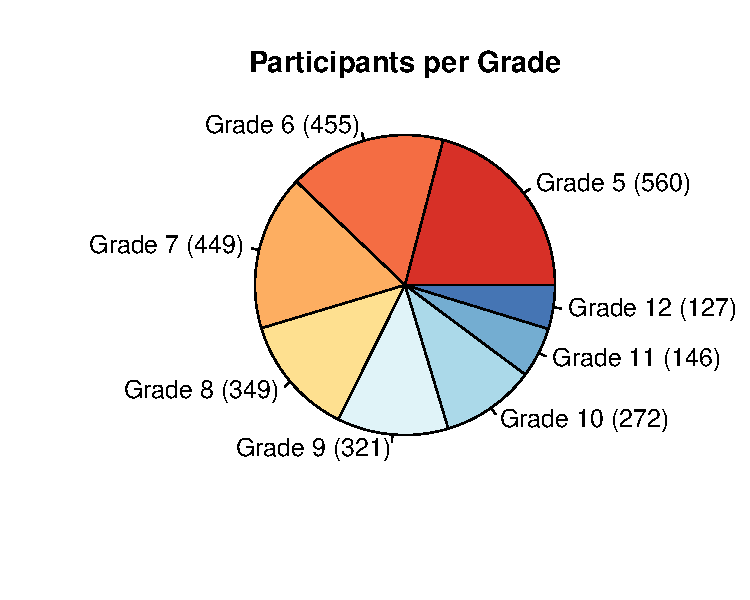
\includegraphics[width=\maxwidth]{figure/minimal-per-class-1} 

}



\end{knitrout}

\subsection{Dalība un sociāli-ekonomiskie rādītāji}

% Trīs 14-bumbulīšu diagrammas

Šeit varētu ievietot diagrammas pa novadiem vai novadu grupām, kas parāda divu parametru attiecību (varētu būt runa par burbulīšu diagrammām, ko zīmē divās dimensijās; turklāt burbulīša laukums ir aptuveni proporcionāls skolēnu skaitam olimpiādē).

\begin{itemize}
\item Sociāli-ekonomisko rādītāju --- bezdarbu, IIN uz 1 iedzīvotāju, pašvaldības izdevumus uz 1 skolēnu vai skolēnu skaitu skolā.
\item Dalībnieku aktivitāti (dalībnieku attiecību pret visiem skolēniem novadā) kā arī olimpiādes summāro rezultātu (punktu summas attiecību pret visiem skolēniem novadā). 
\end{itemize}

Šādas diagrammas palīdzētu saprast, kādi sociālie priekšnoteikumi veicina interesi par olimpiādēm, kāda izglītības politika (piemēram, mazo skolu saglabāšana vai slēgšana; lielāki vai mazāki izdevumi par vienu skolēnu) varētu pozitīvi iespaidot olimpiāžu rezultātus. 



\section{Vidējie rezultāti dalībnieku kategorijām}


%% Visu dalībnieku darbi, iekrāsotas godalgotās vietas 
%% Meiteņu un zēnu darbi (Meitenes zīmējam tanī pašā histogrammā)
%% Meitenes ir sazīmētas apakšā. 

%% Urbaniz. tips. Rīgas, 8 lielo pilsētu, mazpilsētu un lauku darbi

%% Latviešu un krievu valodā rakstītie darbi

%% Latviešu un krievu valodā rakstītie darbi -- tikai 9 lielajās pilsētās




\subsection{``Nevienlīdzība'' un Džini koeficienti}

Viegli redzēt, ka skolēnu izredzes olimpiādē būtiski atšķiras no izvēlētā matemātikas skolotāja, skolas un arī no pašvaldības. Šajā apakšnodaļā mē\v{g}ināsim saprast, cik lielā mērā varbūtība piedalīties olimpiādē, izredzes iegūt godalgotu vietu (mūsu aprēķinos --- atrašanās augšējā kvartilē) un arī iegūtais punktu skaits ir sadalīti nevienlīdzīgi starp skolotāju audzēkņiem. Ņemot vērā to, ka labākie olimpiāžu rezultāti ir sakoncentrēti nedaudzās skolās, šādu nevienlīdzību nevar pilnībā izskaidrot ar skolotāju prasmēm vien, bet gan ar bērnu atlasi.  

\noindent
{\bf Atskaites punkts: Skaitliska ``vienlīdzības'' simulācija.} Protams, pilnīga vienlīdzība nav nedz sasniedzama, nedz arī vēlama. Lai Džini koeficientu aprēķinam rastos kāds atskaites punkts, izdarīsim virkni pieņēmumu par to, kā izglītība ir organizēta hipotētiskā valstī Aizspogulijā, kur ir līdzīga skolēnu un skolotāju demogrāfija, bet olimpiādes rezultāts atspoguļo vienīgi skolēnu matemātiskās spējas. Ja mums rastos iespēja salīdzināt Latvijā pastāvošo rezultātu nevienlīdzību ar kādu reālu valsti, tad Aizspoguliju varētu aizstāt ar kādu reālu piemēru.

\begin{itemize}
\item Aizspogulijā dzīvo 120000 skolēnu, kas mācās no 5.\ līdz 12.\ klasei. 
\item Katra Aizspogulijas skolotāja vai pulciņa vadītāja pārraudzībā esošo skolēnu skaits ir nejaušs, vienmērīgi sadalīts vesels skaitlis no 0 līdz 100. (Pavisam Aizspogulijā ir 2400 matemātikas skolotāju --- vidēji pa vienam uz katriem 50 skolēniem.)
\item Aptuveni 2\% no Aizspogulijas skolēniem vēlas piedalīties matemātikas olimpiādē. 
\item Visā Aizspogulijā skolēniem ir līdzīgas iespējas sagatavoties olimpiādei, olimpiādes rezultāts atspoguļo nevis skolotāja, skolas vai pašvaldības izvēli, bet ir atkarīgs no skolēna dotumiem (matemātiska apdāvinātība, spēja pierakstīt risinājumus, mērķtiecīga gatavošanās, utml.) Olimpiādē saņemtie punkti ir sadalīti ar {\em nogriezto normālo sadalījumu} ({\em truncated normal distribution}) ar vidējo vērtību $\mu = 15$, standartnovirzi $\sigma = 10$ un vērtībām intervālā $[0,50]$.
\item Jebkuram skolēnam ir vienādas izredzes nokļūt pie jebkura skolotāja; nenotiek skolēnu stratifikācija atkarībā no mācību rezultātiem. 
\end{itemize}

Šajā piemērā Aizspogulijas skaitliskie lielumi (skolēnu un matemātikas skolotāju skaits; punktu sadalījums olimpiādē) aptuveni atbilst Latvijas situācijai, tomēr nepastāv skolēnu šķirošana. Aizspogulijas rādījumus Džini koeficientam ņemsim par atskaites punktu, lai varētu salīzināt, par kādu daļu Latvijā pastāvošās iespējas gatavoties olimpiādēm ir nevienlīdzīgākas. (Nebūtu jēgas salīdzināt ar Džini koeficientu 0, jo tas nozīmētu olimpiāžu dalībnieku un viņu punktu absolūti vienādu sadalījumu starp skolotājiem, kas ir mazticami pat ar Aizspogulijas pieņēmumiem.) 

To nevienlīdzību (pareizāk sakot - galaiznākumu nevienādību), kas rodas Aizspogulijā varbūtisko sadalījumu ieviesto nejaušību rezultātā iegūsim, izmantojot skaitlisku olimpiādes rezultātu simulāciju. Katram no 2400 skolotājiem piešķiram nejaušu skolēnu skaitu no 0 līdz 100; katrs skolēns piedalās Bernulli eksperimentā (ar varbūtību 2\% piedalās olimpiādē); visbeidzot katrs olimpiādes dalībnieks iegūst punktu kopskaitu atbilstoši nogrieztajam normālajam sadalījumam. Šādi iegūtajiem datiem aprēķinām tās pašas Lorenca līknes un Džini koeficientus.


\noindent
{\bf Lorenca līkne dalībnieku skaita, augšējās kvartiles dalībnieku skaita un punktu summas sadalījumam starp skolotājiem Aizspogulijā (olimpiādes rezultātu vietā skaitliska simulācija):}

\begin{knitrout}
\definecolor{shadecolor}{rgb}{0.969, 0.969, 0.969}\color{fgcolor}

{\centering \includegraphics[width=\maxwidth]{figure/minimal-gini2-1} 

}



\end{knitrout}


\begin{knitrout}
\definecolor{shadecolor}{rgb}{0.969, 0.969, 0.969}\color{fgcolor}
\begin{tabular}{l|r}
\hline
Measurement Type & Gini for Looking-Glass Land\\
\hline
Participants & 0.277\\
\hline
Q3 & 0.655\\
\hline
Points & 0.370\\
\hline
\end{tabular}


\end{knitrout}


Aizspogulijas simulācijā ir ievērojama nevienlīdzība starp to, cik potenciālos olimpiāžu laureātus (risinātājus, kuru rezultāts ir augšējā kvartilē) sagatavotu katrs skolotājs. Ja skolotāju iesaiste olimpiādē ir līdzīgāka un vidējais audzēkņu skaits uz vienu skolotāju ir mazāks, tad ir pašsaprotami, ka liela daļa no viņiem nesagatavos nevienu laureātu. No šejienes izriet secinājums, ka skolu darbu nebūtu pareizi salīdzināt pēc sagatavoto olimpiāžu laureātu skaita --- it īpaši, ja mērķis ir izglītības iespēju vienlīdzība. Savukārt, salīdzinājums pēc olimpiādes dalībnieku skaita un arī olimpiādē savākto punktu skaita ir pilnīgi adekvāts: šie ir rādījumi, kurus ikviena skola var uzlabot neatkarīgi no citām. Pat ar pieņēmumu, ka tikai aptuveni 2\% skolēnu vēlas piedalīties atklātajās matemātikas olimpiādēs. 

\section{Atsevišķo uzdevumu vērtējumi}

\subsection{Vidējie vērtējumi}

Vidējo vērtējumu uzdevumam $X = \{ x_i \}$ aprēķina pēc formulas: 

\[ E(X) = \frac{\sum_{i=1}^{n}{x_i}}{n}, \]

\noindent
kur $x_i$ ir $i$-tā skolēna vērtējums par uzdevumu $X$, bet $n$ ir visu attiecīgās klases darbu skaits: $n = \left| X \right|$.

\subsection{Šenona entropija}

Entropiju uzdevuma $X$ vērtējumiem aprēķina pēc formulas:

\[ H(X) = - \sum_{i = 0}^{10}{p_i}\cdot \log_2{p_i}, \]

\noindent
kur $p_i = \frac{\left|\{ x \in X | x = i \}\right|}{\left| X \right|}$ ir varbūtība saņemt par uzdevumu $X$ vērtējumu $i$ (piemēram $p_0$ - vērtējumu "0 punkti" vai "uzdevums nav risināts" dalījums ar visu attiecīgās klases darbu skaitu). Ja kāds no vērtējumiem $i$ par attiecīgo uzdevumu nav sastopams, tad attiecīgo saskaitāmo entropijas formulā izlaiž.

Augsta entropija nozīmē augstu nenoteiktību. Ja visi vērtējumi par attiecīgo uzdevumu būtu vienādi, tad entropija ir 0. Ja visi vērtējumi no 0 līdz 11 ir vienādi bieži sastopami, tad entropija ir $\log2(11) \approx 3.46$. Pārāk zema entropija (piemēram tuvu 1 vai mazāka) nozīmē to, ka pats uzdevums vai tā vērtēšanas sistēma nav bijuši pārāk noderīgi olimpiādes dalībnieku punktu skaita diferencēšanai, jo pārāk daudzi vērtējumi ir vienādi.


\subsection{Korelācija ar pārējiem uzdevumiem}

Izvēļu testu ({\em multiple choice exams}) analīzē bieži izmanto {\em biseriālo korelācijas koeficientu} --- kāda ir korelācija starp eksāmena kopīgo rezultātu un atbildēm (pareizas/nepareizas) uz konkrēto uzdevuma jautājumu. Ar šo skaitlisko kritēriju var atrast tos testu jautājumus, kuri varētu būt mulsinoši formulēti vai arī nemēra tās pašas prasmes, ko citi šī paša testa uzdevumi. 

Protams, olimpiāde nav izvēļu tests (un par katru no jautājumiem ir vairāk vērtējumu nekā tikai 0 vai 1). Tomēr arī šajā gadījumā korelācija var noderēt. Ja uzskatām, ka olimpiāde kopumā mēra noteikta veida matemātiskas prasmes, tad par katru uzdevumu var uzdot jautājumu: Cik labi šis uzdevums palīdz mērīt to pašu, ko olimpiādes uzdevumu komplekts kopumā? Ja konkrētais uzdevums labi ``iederas'' starp citiem, tad korelācija būs augsta, ja tas mēra kādas stipri atšķirīgas prasmes nekā citi tās pašas klases uzdevumi, tad korelācija būs mazāka. Korelāciju rēķina pēc šādas formulas:

\[ \mbox{cor}(X,Y) = \frac{\sum_{i=1}^{n}{x_i y_i} - n \cdot E(X) \cdot E(Y)}{\sqrt{\sum_{i=1}^{n}{x_i^2} - n \cdot E(X)^2} 
\cdot \sqrt{\sum_{i=1}^{n}{y_i^2} - n \cdot E(Y)^2}}, \]

\noindent
kur $x_i$ ir $i$-tā dalībnieka vērtējums par uzdevumu $X$, $y_i$ ir vērtējumu summa par visiem 4 atlikušajiem uzdevumiem, $n$ --- darbu skaits attiecīgajā klasē, $E(X)$ apzīmē $x_i$ aritmētisko vidējo.

Korelācijas koeficients vienmēr ir intervālā $[-1,1]$. Teorētiski varētu gadīties arī negatīva korelācija, t.i. tāds uzdevums, kuru veiksmīgākie olimpiādes dalībnieki risināja sliktāk nekā mazāk veiksmīgie. Tad paša uzdevuma vai vērtēšanas sistēmas korektums radītu nopietnas šaubas. Olimpiāžu praksē tomēr negatīvas korelācijas nav vērojamas. Salīdzinoši zemas uzdevuma vērtējuma korelācijas ar citiem uzdevumiem ļauj atrast tos uzdevumus, kuru tēma vai vērtēšanas kritēriji ir būtiski atšķīrušies no citiem uzdevumiem tajā pašā klases 5 uzdevumu komplektā.

\subsection{Vērtējumu atšķirības zēniem un meitenēm}

Vērtējumu atšķirību konkrētas klases uzdevumam $X$ aprēķina kā divu vidējo vērtību starpību: 

\[ \Delta_{\mbox{gender}}(X) = E\left(X_{\mbox{male}}\right) - E\left(X_{\mbox{female}}\right), \]

\noindent
kur $X_{\mbox{male}}$ ir visi attiecīgās klases zēnu vērtējumi un  $X_{\mbox{female}}$ ir attiecīgās klases meiteņu vērtējumi, un $E(X)$ - skaitļu virknes $X$ aritmētiskais vidējais.

Katram no uzdevumiem atrasta zēnu un meiteņu vidējo vērtējumu starpība. Pozitīvs skaitlis nozīmē to, ka zēnu vērtējums bija augstāks, negatīvs skaitlis --- to, ka meiteņu vērtējums bija augstāks.



\end{document}
